\chapter{Development}
The first necessarily step to the development of the work is make the abstractions, for that we classify and separate the entities, relationships and attributes of work. The data base is composed by a couple of entities called by “Social Media” and "Person", a couple types of relationship, the "HAS" to connect one person to a social network, and another relationship to represent connections type between the social networks, as the possible following labels: "PERSONAL", "INFLUENCE", "PROFESSIONAL\_RELATIONSHIP", e "CONTENTS".

Such abstractions that were citated anteriorly are codified in a program that automatize the insertion process and population of Neo4J, applying some validations and a defined logic to several connections as the verification of a relationship type, and can be find at the following \href{https://github.com/LeonardoLeiteMeira/process_CSV_to_graph_database}{repositório}. To use is necessary substitute connections data of Neo4J to the local machine.



\section{Social Medias}

The Social Media is responsible for represent one social network of one single person. A social network can be connected to many other social media and in just one person. By this way, the social networks that were chosen to be part of the project initially are currently the main utilized, being them the Instagram, Facebook, Ticktok, Youtube, Pinterest e Twitter.
The attributes of each social network are

\begin{itemize}

\item Identifier: Single identifier of the entity

\item Name: Social network name that the entity refers to 

\item User name: Responsible for identify the user name chosen by 
the person that created that social network

\item Identifier of the user: Responsible for being a reference to a person identifier ("Person" entity")

\end{itemize}




\section{Person}

The “Person” entity represent the person that utilize determinated social networks. One person can be related to many others different social networks, and yours relations with another people happen through those social networks. 

One instance of the “Person” entity have the following attributes:

\begin{itemize}
\item Identifier: A single identifier to that user
\item Name: User’s first name
\item Surname: User’s last name
\end{itemize}


\section{Relationships}


The relationships between the entities describe the behavior that are being charted by the graphs, in this case exist a couple type of present relationship at the system, one to represent the connection between one person and you social networks and another one to represent the connections between the social networks.

The first relation, between one person and tour social networks are described for the vertice “Has”, each person must be in a social network set. Were the connection are defined based at this relation. The image 3.1 shows the relation of the “Alice” person with your social networks through the vertice "HAS".  

\begin{figure}
    \centering
    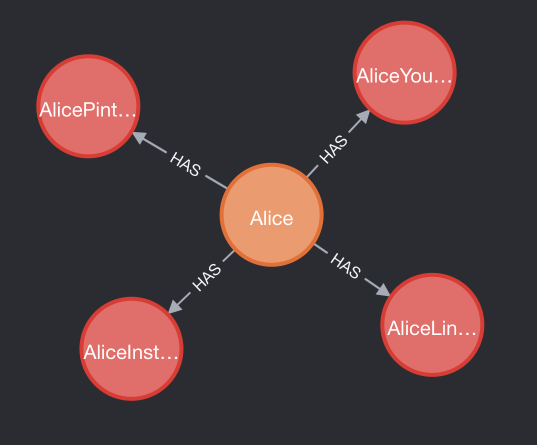
\includegraphics[scale=0.5]{alice}
    \caption{"Alice" entity with the vertices for your social networks}
    \label{fig:my_label}
\end{figure}



The other type of relationship would be one that describes the connection between two social networks of different people. This relationship takes into account the type of connection and the social networks used by two users, and can be of the following types:

\begin{itemize}
    \item Personal: Follow each other on networks for personal use
    \item Professional: Follow each other in professional networks
    \item Content consumption - Follow each other on networks focused on video content
    \item Influence: Represents the relationship of influence, when a person does not follow another but is followed by him. The vertical arrow points to who is followed, that is, who influences the relationship.
\end{itemize}



In figure 3.2 it is possible to visualize the entity "Alice" linked to the social network "AliceInstagram", and its relationship with other social networks of other people.

\begin{figure}
    \centering
    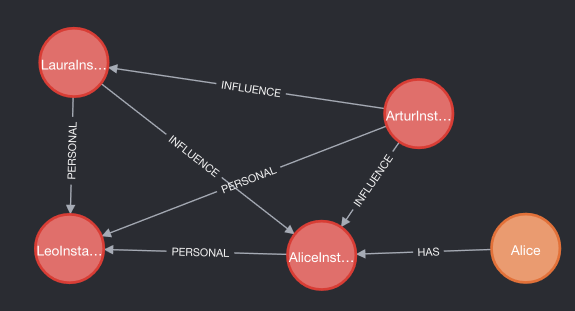
\includegraphics[scale=0.5]{imagens/alice_others.png}
    \caption{
Entity “Alice” with its social network connecting to other networks}
    \label{fig:my_label}
\end{figure}

\section{Queries}

Given the database structure presented and the objectives of this work, some queries were created in Cypher to return the desired information. The querie below returns the social media of a given person. In the example, you are looking for a person's social networks with the "Name" property as "Laura".
\begin{verbatim}
match(person:Person {Name: "Laura"})-[HAS]->(socialMedia:SocialMedia) 
return socialMedia
\end{verbatim}


The next query is intended to return all people connected to someone else's social networks. In the example, the query is looking for people connected to a person's social networks with the "Name" property as "Laura".

\begin{verbatim}
match(p:Person{Name:"Laura"})-[]-(s:SocialMedia)
match(s)-[]-(sl:SocialMedia)
match(sl)<-[HAS]-(f:Person)
return f
\end{verbatim}

The following query looks for the first-level connections for a relationship type. In the example, it searches for people who have a social network (in this case, instagram), then it searches for the social networks connected in a type of relationship (in the example, the relationship is "PERSONAL"), and finally, it searches for the social networks connected to a person (in the Leonardo case). With this query it is possible to list all connections for a type of relationship that has been identified.

\begin{verbatim}
match (p:Person)-[]-(s:SocialMedia{Name:"Instagram"})
match (s)-[f:PERSONAL]-(sl)
match (sl)-[:HAS]-(se:Person{Name:"Leonardo"})
return p
\end{verbatim}

The following query performs an in-depth search using the plugion APOC \cite{apoc} available in the Neo4J system. In the first line, the social network with “Name” defined as “Instagram” of the person “Alice“ is selected. In the second line, the search for node S (Alice's Instagram) begins, then the search for vertices is performed, with a maximum depth of 5. The result of this query are the suggestions of possible new connections of a personal nature that can be made .

\begin{verbatim}
match (p:Person{Name:"Alice"})-[]-(s:SocialMedia{Name:"Instagram"})
call apoc.path.spanningTree(s,{relationshipFilter: "PERSONAL",minLevel:0,maxLevel: 5})
YIELD path
RETURN path, p;
\end{verbatim}

For other types of recommendations just replace the "relationshipFilter" property to "INFLUENCE", to have influence recommendations, to "PROFESSIONAL\_RELATIONSHIP" to have professional connection recommendations, or "CONTENTS" to have content recommendations.


The following query is intended to return the influence score that a given person has. In the example below, all of a person's social networks are selected, in this case "Alice", and then the number of influence connections is returned.

\begin{verbatim}
match(person:Person {Name: "Alice"})-[HAS]->(socialMedia:SocialMedia)
match(socialMedia)<-[f:INFLUENCE]-()
return count(f)
\end{verbatim}


This last query aims to identify someone's level of influence within a network. In the first line, the social networks of a person are selected to be evaluated for influence. In the second line, all the social networks of a network that must be evaluated, which are influenced are selected, and finally it is defined which network the level of influence is being evaluated, in this case a social network with the property "Username" with the value " LauraInstagram”.
\begin{verbatim}
match(person:Person {Name: "Leonardo"})-[HAS]->(socialMedia:SocialMedia)
match(socialMedia)<-[f:INFLUENCE]-(socialMediaInOtherSubGraph:SocialMedia)
match(socialMediaInOtherSubGraph:SocialMedia)-
    []-(subGraph:SocialMedia{Username:"LauraInstagram"})

return count(f)
\end{verbatim}





